\chapter{Testing}
\label{ch:testing}
\section{Introduction}
\newpage

\begin{landscape}
	\section{Requirements Testing}
	\begin{tabularx}{\hsize}{lllXr}
		\toprule
		ID & Name & Expected Output & Evidence & Success? \\
		\midrule
		F1 & User Interaction 
		& A page should display to allow the user to interact with the bot
		& 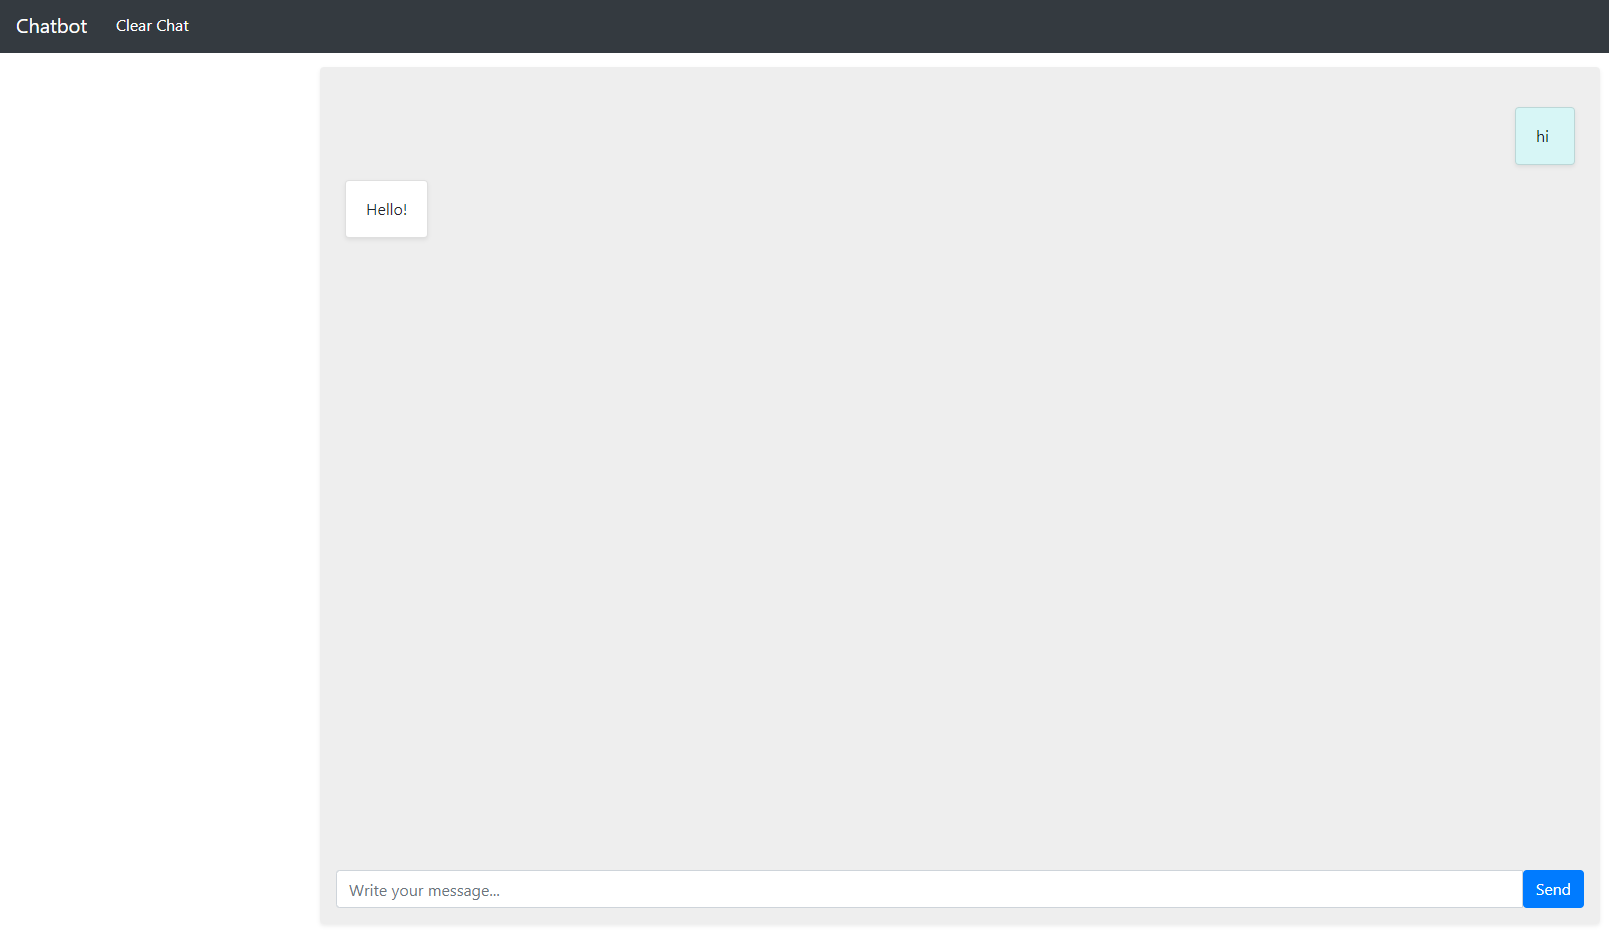
\includegraphics[width=8cm]{tests/f1} & Yes \\
		\midrule
		F2 & Browser Access
		& The user should be able to access the system via a browser
		& 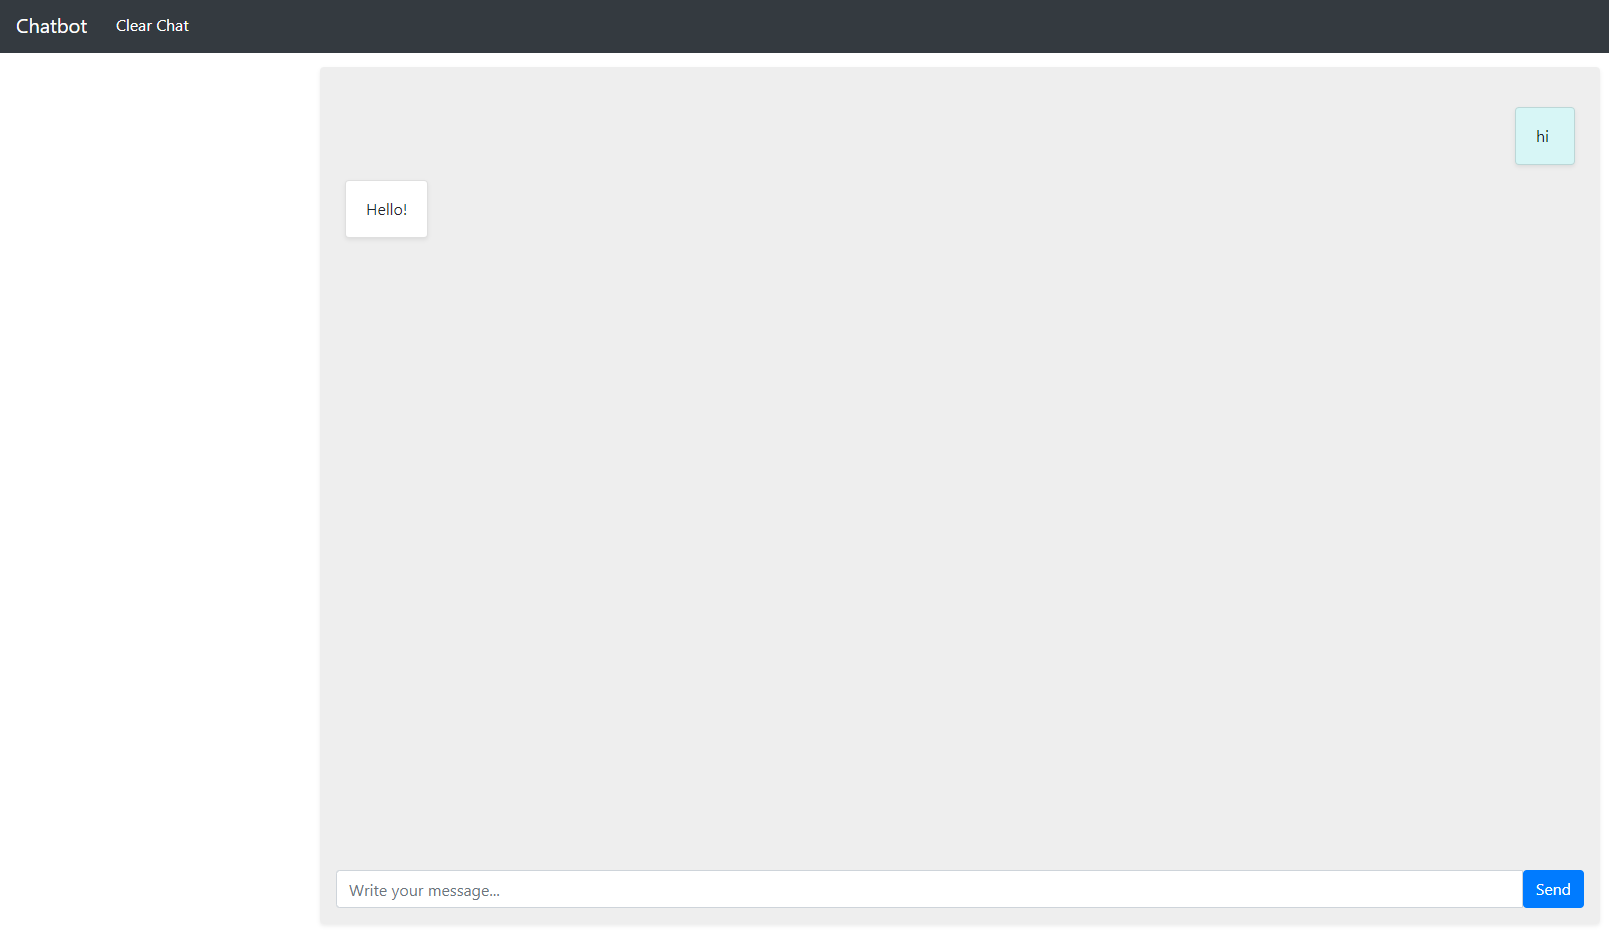
\includegraphics[width=8cm]{tests/f1} & Yes \\
		\midrule
		F3 & User Input
		& The user should be enter queries to the bot using a textbox input
		& 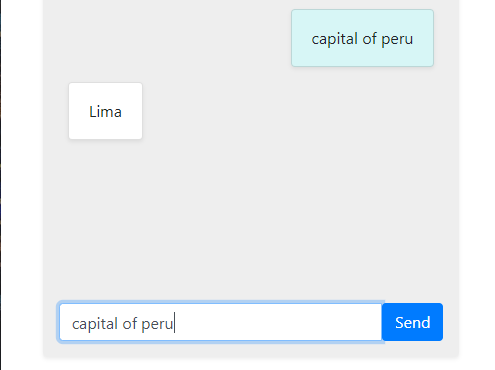
\includegraphics[width=8cm]{tests/f3} & Yes \\
		\bottomrule
		F4 & Responses on Page
		& The should see the chatbot response on the web page
		& 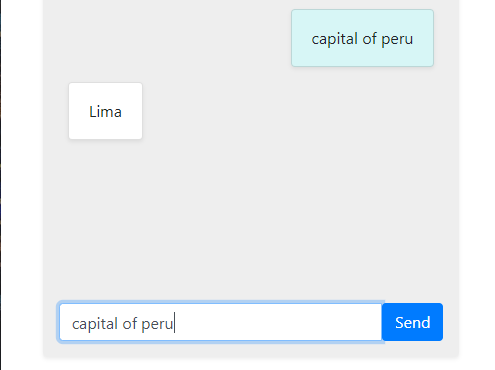
\includegraphics[width=8cm]{tests/f3} & Yes \\
		\bottomrule
		F5 & Conversation history
		& The should see the whole conversation with the bot on the page
		& 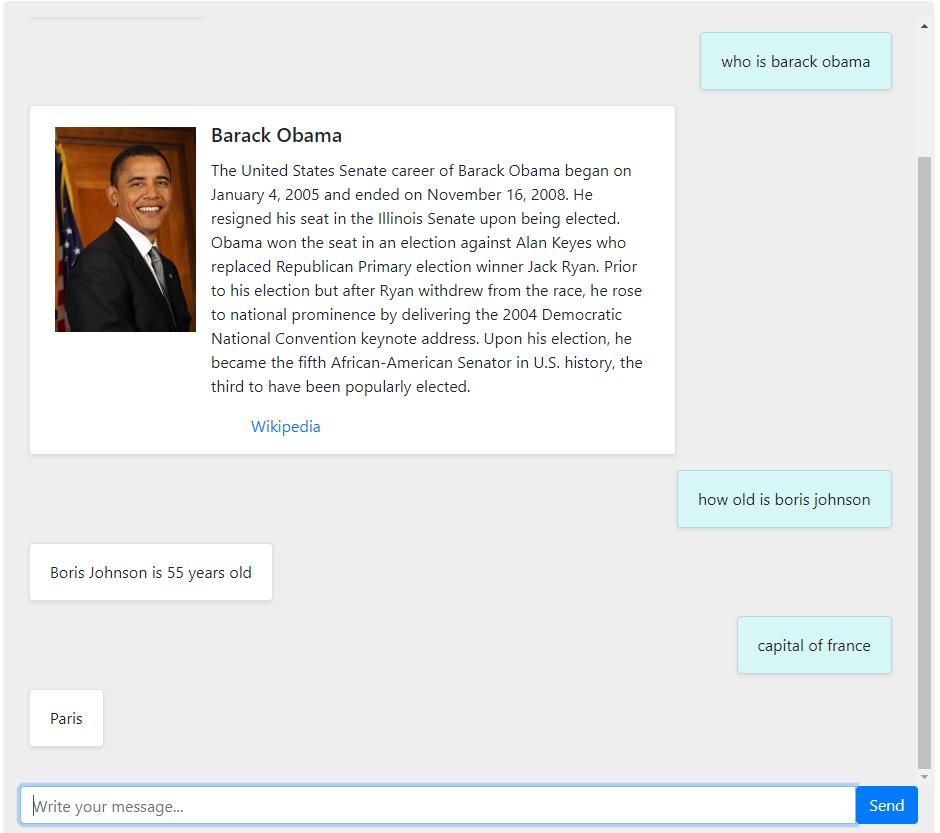
\includegraphics[width=8cm]{tests/f5} & Yes \\
		\bottomrule
		%\caption{Requirements testing and evidence}
		%\label{tab:testreq}
	\end{tabularx}
\end{landscape}


\newpage
\section{Unit Testing}
\section{User Acceptance Testing}
\section{Conclusion}